%% This is the main content about this article. I should list them in an order
%% How to balance the existing model, positive and negative instance together, I shall use the dfg-method to create a dfg-matrix to incorporate the impact.
%% how to introduce them into adding long-term dependency feature. After mining the model by Inductive Miner, we have a model without long-term dependency, but we need to change the model and give the right examples.. 
%% If we change the data set, then we need to change the model into another parts, but the current methods can not solve it..
%% Should we also separate them into different sections?? Yes, we need it
%% Also, to delete the silent transition, as one option feature in our methods, we only delete it, in this situation, which will not affect the model behavoirs.

%% Or we could organize the content in this way:
%%  -- put the whole structure ahead and put all that we want to talk
%%  -- list the steps 
%%    ++ dfg-method to balance the directly-follows relation and create the corresponding directly-follows graph
%%    ++ add long-term dependency on the model
%%    ++ delete the silent transitions on the model as a post model

%% Put some words here
This chapter begins with a general framework to repair a reference process model by incorporating the negative instances. A concrete algorithm within the framework is proposed in the subsequent sections. 
%our repair algorithm to incorporate the negative instances on process enhancement. In the beginning, the architecture of this algorithm is provided to give an overview. Details of main steps are represented in the following order. Firstly, the impact of the existing model, positive and negative instances are balanced in the media of the directly-follow relations. Inductive Miner is then applied to mine process models from those directly-follows relations. Next, we detect and add long-term dependency on the generated process models. Furthermore, the model in Petri net with long-term dependency is  post-processed for the sake of simplicity. 
\section{General Framework for Repairing Process Models}
%% Describe the 
Figure \ref{fig:framework} shows our proposed framework to repair a process model with negative information. The inputs are a reference process model and a labeled event log. The reference process model can be in multiple types, e.g. Petri net, process tree. Traces in the labeled event log are classified as positive or negative in respect to some KPIs of business processes. The output is a repaired process model with the same type as the reference model.

The basic idea behind the framework is to unify the impact from the reference model $M$, positive sublog $L^+$ and negative sublog $L^-$ into data models. Those data models are of the same type and denoted as $D^M$, $D^+$ and $D^-$ respectively. Then we consider all impact from models and generate a new data model $D^n$. $D^n$ is later transformed into a process model $M^r$ as the output. Several post-processes are optional to improve the repaired model $M^r$.

After defining a data model to unify the impact and implementing the process modules in the general framework, we propose a concrete solution which also considers the negative information on model repair. 
\begin{figure}
	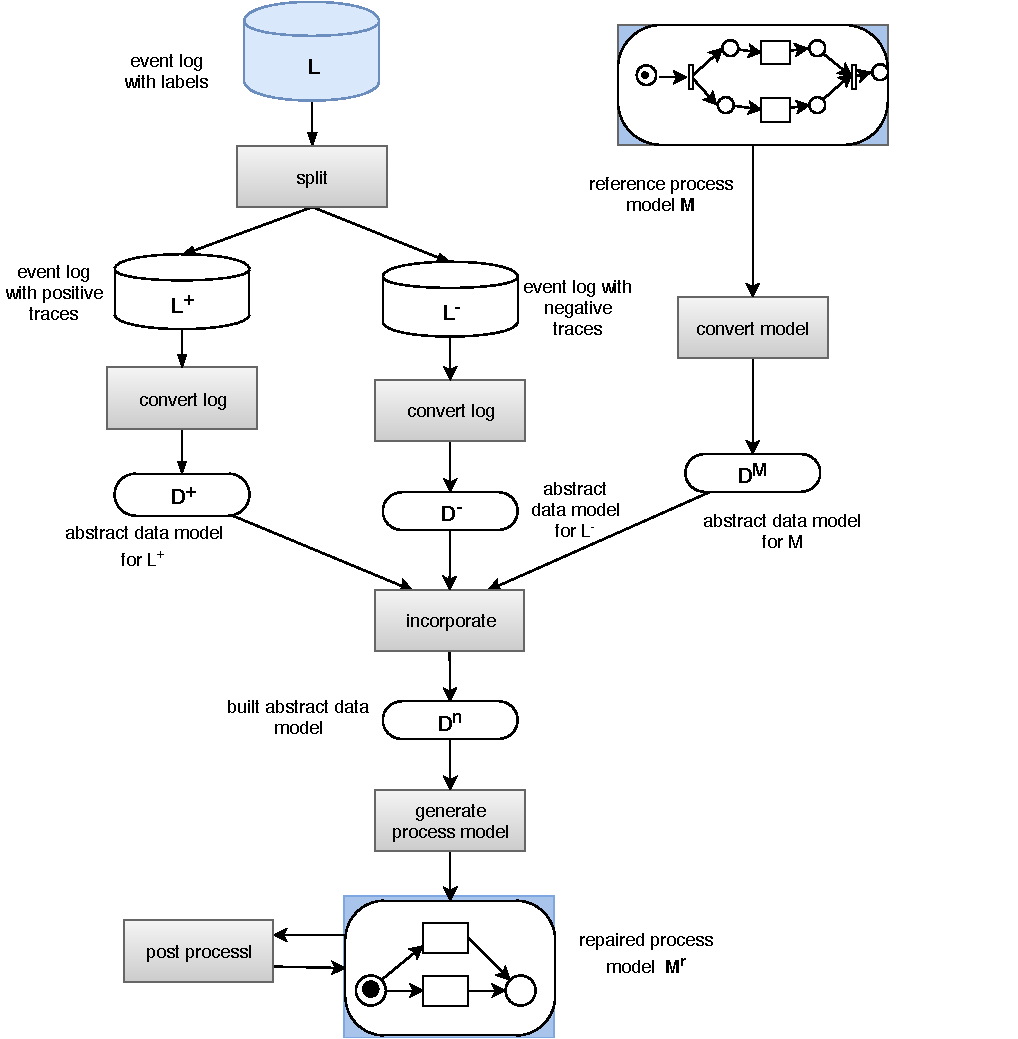
\includegraphics{figures/algorithm/FD_framework.pdf}
	\caption[Model Repair Architecture]{Model Repair Architecture -- \small Rectangles represents processes and data models in eclipse shape. Input event log and the reference model are in blue, while the repaired model is in green.}
	\label{fig:framework}
\end{figure} 
\section{Algorithm}
Given the inputs, an event log and a Petri net as the reference process model M as shown in Figure \ref{fig:scope}, our task is to repair the referenced Petri net based on the actual event log with consideration of negative information. 

Based on this scope, the main modules in the framework in Figure \ref{fig:framework} are designed and developed to repair the reference Petri net. We denote our repair algorithm as \textbf{dfg-repair}. First of all, we define a proper data model to represent the impact from Petri net M, and the event log L. Then, we list all the modules  and describe our basic ideas to implement them. 
% here to point out our input and output
\subsection{Unified Data Model}
We choose the directly-follows graph as the basis of our unified data model to represent the impact from the reference model and the event log. The reasons are, (1) there exist transformation algorithms to extract a directly-follows graph from an event log and to convert directly-follows graph into process tree or Petri net, which saves the development effort by reusing them;(2) the cardinality of directly-follows graphs can be used to express the impact strength.

Although we can derive three directly-follows graphs from the reference model, the positive and negative event logs respectively, their cardinalities are in different level. Therefore, to incorporate those graphs together, we introduce a concept called unified cardinality to bring all the impact onto the same level, which is the percentage to the sum of total cardinalities with a range [0-1].
% here we already changed the definitions for the unifications..now it became as the percentage of the cardinality to its whole cardinality. No matter negative or positive ones...we can do it, right? 
\begin{definition}[Unified cardinality] 
	\label{def:car-unification}
	Given a directly-follows graphs $G(L)  = (A, F , A_{start}, A_{end})$ for a model, the unification for this graph is a function  $u:F\rightarrow \mathbb{R} $ that has the following definition: \\
	for each directly-follows relation $(a,b) \in F$,
	\[ u(a,b) = \frac{c(a,b)}{\sum_{(a^\prime,b^\prime) \in F} c(a^\prime,b^\prime)}\]
	for start activities $a \in A_{start}$, 
	\[ u(a) = \frac{c(a)}{\sum_{a^\prime \in A_{start}} c(a^\prime)} \]
	Similarly for end activities $a \in A_{end}$,
	\[ u(a) = \frac{c(a)}{\sum_{a^\prime \in A_{end}} c(a^\prime)} \]
\end{definition}
A directly-follows graph with unified cardinality is denoted as a unified directly-follows graph $D(L)=(A, F , A_{start}, A_{end}, u)$. After analyzing the positive, negative instances from event logs and the reference process model, $D(L_{pos})$, $D(L_{neg})$ and $D(L_{ext})$ are generated as the directly-follows graphs with unified cardinalities.
\subsection{Modules List}
After fixing the unified data models, in order to repair the reference model, the following list of modules are necessary. 
% should we add some steps here to say from which model to which model??
\begin{itemize}
	\item \emph{Split event log into positive and negative sublogs } \quad
	The event log $L$ is split into an event log $L^+$ with only positive traces and an event log $L^-$with negative traces.
	\item \emph{Convert event logs into unified directly-follows graphs, $D^+, D^-$}\quad 
	Two unified directly-follows graphs are generated respectively for the positive instance and negative instances from the event log.
	\item \emph{Convert reference model into unified directly-follows graph $D^M$}\quad 
	\item \emph{Incorporate unified directly-follows graphs} \quad
	Three unified directly-follows  graphs $D^M, D^+, D^-$ are combined into one single directly-follows graph $D^n$ after balancing their impact.
	\item \emph{Generate process models from $D^n$} \quad
	Process models are mined from the repaired data model $D^n$.
	\item \emph{Post process the repaired model} \quad
	Several post-processes are optionally applied on the generated process model, in order to improve the process model quality according to certain criteria.
	%Long-term dependency is detected on the intermediate models and finally added on the Petri net. To simplify the model, the reduction of silent transitions can be applied at the end.
\end{itemize}
Among those modules, for simplicity, we skip the details for the module \emph{Split event log into positive and negative sublogs}. The details of the concrete algorithms to implement other modules are provided in the subsequent sections.
\subsection{Convert Event Logs into Unified Directly-follows Graphs}
Given an event log, to retrieve its unified directly-follows graph, we need to obtain its directly-follows graph at first. There is an existing procedure \emph{IMLog2Dfg} from  \cite{leemans2013discovering}. \emph{IMLog2Dfg} traverses traces in the event log, extracts directly-follows relations of activities, and generates a directly-follows graph based on those relations. 

By applying \emph{IMLog2Dfg} separately on the event logs $L^+$ and $L^-$, we generate two directly-follows graphs $G(L_{pos})$ and $G(L_{neg})$.  In the next step, the cardinalities from those graphs are unified according to Definition \ref{def:car-unification} and become a part of unified data model $D(L_{pos})$ and $D(L_{neg})$

\subsection{Convert Reference Model into Unified Directly-follows Graph}
The basic idea behind this convert is to transform a reference process model into a directly-follows graph and then unify this directly-follows graph into $D^M$.


To generate a directly-follows graph from a Petri net, we investigate the execution order of activities with help of a transition system. % how ti helos
In a transition system, the set of activities directly before a state have to be executed to reach this state, while the activities after this state are enabled to execute only after reaching this state. This implies the set of the activities before the state is executed before the set after the state. By analyzing the transition system, directly-follows relations between activities are extracted and used later to a directly-follows graph for the reference model.

From the positive and negative event logs, we can get the cardinality for corresponding directly-follows graph to represent the strength of this directly-follows relation. However, when the existing model is transformed into  directly-follows graph $G(L_{ext})$, there is no point to assign cardinality on each edge. So we just set cardinality with 1 for each arc. Based on this cardinality assignment, we attain the unified data model $D^M$ for the reference Petri net.

\subsection{Incorporate Unified Directly-follows Graphs}
After the unification, the impact from the existing model, the impact from positive and negative instances are in the same level and represented in $D^M$, $D^+$, and $D^-$. 
The strategy to incorporate those three models is that directly-follow relations are added into the repaired data model $D^n$ if the total support from $D^M$ and $D^+$ exceeds the rejection force from $D^-$. The other directly-follows relations are rejected. Namely, we balance all impact by subtracting the unified cardinality of $D^-$ from the sum of unified cardinality in $D^M$ and $D^+$.
\begin{definition}[Incorporating method] For any directly-follows relation from $D^M$, $D^+$, and $D^-$, we balance all forces on it in the following way. 
	\begin{itemize}
		\item For one directly-follows relation, \[ u^{n}(a,b) =  u^{M}(a,b)+ u^{+}(a,b)  - u^{-}(a,b) \] 
		\item For a start activity $a \in A^{M}_{start} \cup A^{+}_{start} \cup A^{-}_{start}$,
		\[ u^{n}(a) =  u^{M}(a)+ u^{+}(a)  - u^{-}(a)\]
		\item For an end activity $a \in A^{M}_{end} \cup A^{+}_{end} \cup A^{-}_{end}$
		\[ u^{n}(a) =  u^{M}(a)+ u^{+}(a)  - u^{-}(a)  \]
	\end{itemize}	
%if $u^{n}(a,b) > 1 , u^{n}(a,b) =1$, if $u^{n}(a,b) < 0 , u^{n}(a,b) =0$; 
% $ u^{n}(a) > 1 \Rightarrow  u^{n}(a) =1 ; u^{n}(a) < 0 \Rightarrow  u^{n}(a) =0$;
\end{definition}
% here is only the incorporation method
%% Here we add the control weight on it
In real life, there exists various needs to address the impact either from the existing model, the positive instances or the negative instances. To meet this requirement, three control parameters $w^{M}$, $w^{+}$, and $w^{-} \in [0,1]$ are assigned respectively to each unified cardinality from the existing model, and positive and negative instances. The weighted unification is modified in the way bellow. 
\begin{definition}[Weighted incorporating method]
Given the control weight $w^{M}$, $w^{+}$, and $w^{-} \in [0,1]$, the weighted incorporating method to balance forces from $D^M$, $D^+$, and $D^-$ for $D_{n}$ is defined below.
\begin{itemize}
	\item For one directly-follows relation, \[ u^{n}_{w}(a,b) =  w^{M} \cdot u^{M}(a,b)+ w^{+} \cdot u^{+}(a,b)  - w^{-} \cdot u^{-}(a,b) \] 
	\item For a start activity $a \in A^{M}_{start} \cup A^{+}_{start} \cup A^{-}_{start}$,
	\[ u^{n}(a) =  w^{M} \cdot u^{M}(a)+ w^{+} \cdot u^{+}(a)  - w^{-} \cdot u^{-}(a)\]
	\item For an end activity $a \in A^{M}_{end} \cup A^{+}_{end} \cup A^{-}_{end}$
	\[ u^{n}(a) =  w^{M} \cdot u^{M}(a)+ w^{+} \cdot u^{+}(a)  - w^{-} \cdot u^{-}(a)  \]
\end{itemize}	
\end{definition}
By adjusting the weights of $w^{M}$, $w^{+}$, and $w^{-}$, different focus can be reflected by the model. For example, by setting $w^{M}=0, w^{+}=1, w^{-}=1$, the existing model is ignored in the repair, while  the original model is kept in situation $w^{M}=1, w^{+}=0, w^{-}=0$.

Next, we filter the directly-follows relation according to its weighted cardinality. If the cardinality over one certain threshold, it indicates a significant support to add this relation into the repaired data model $D^n$. By adding those directly-follows relation, we build a unified directly-follow graph $D^n$ over this threshold. 
% here to explain the building method for the new data model and the way from it?? But should we do it here, or later?? 
%After getting the weighted unification, we can assign cardinality for the directly-follows graph $G_{new}$ by multiplying weighted unification with the total number of cardinalities of $G(L_{pos})$, $G(L_{neg})$ and $G(L_{ext})$. 
\subsection{Generate Process Models from $D^n$}
% generate dfg from unified one
% derive models from dfg
The result of the last step above is a unified directly-follows graph $D^n$ with weighted cardinality. To generate a process model from it, we convert $D^n$ firstly into a general directly-follows graph $G^n$. Analyzing the weighted cardinality, we transform the weighted cardinality by multiplying the number of traces of the labeled event log.
%the sum of cardinalities of $G(L^{+})$, $G(L^-)$ and $G(L^{M})$.  

Later, based on $G^n$, an existing procedure called \emph{Dfg2ProcessTree} is applied to mine process models like process tree and Petri net \cite{leemans2013discovering}. It finds the most prominent split from the set of exclusive choice, sequence, parallelism, and loop splits on  a directly-follows graph.  Afterward, the corresponding operator to the split is used to build a block-structured process model called a process tree. Iteratively, the split sub graphs are passed as inputs for the same procedure until one single activity is reached and no split is available. A process tree is output as the mined process model and can be converted into another process model called Petri net.
%% To write the procedure for it 
\subsection{Post Process on the Process Model}
Due to the intrinsic characters of Inductive Miner, the dependency from activities which are not directly-following can not be discovered. To improve precision of the generated model, we propose one post process to add the long-term dependencies to the model. Additionally, another post process to simplify the model is introduced by deleting redundant silent transitions and places.
\subsubsection{Add Long-term Dependency}
Obviously, long-term dependency relates to the structure of choices in process model, such as exclusive choice, loop, and or structure. Due to the complexity of handling long-term dependency on or and loop structure, we skip them but focus only on the long-term dependency in the \textbf{exclusive choice structure}. 

The generated process tree mined by Inductive Miner is used as an intermediate process model to detect long-term dependency.  A process tree is  (1) easy to extract the exclusive choice structure, since it is block-structured. (2) easy to transform a process tree to a Petri net as the final model.
%% Here we need to add the relation of process to the long-term dependency

An exclusive choice structure is represented as \textbf{\emph{xor block}} in a process tree. For the sake of convenience, we name a subtree of an xor block as one \textbf{\emph{xor branch}}. %denote the set of xor blocks B(Q) as and the set of xor branches as BB(Q) for a tree Q.
For two arbitrary xor branches X,Y with long-term dependency, denoted as $ X\rightsquigarrow Y$, they have to satisfy the conditions: 
\begin{itemize}
	\item they have a sequential order;
	\item they have significant correlation. In this thesis, we assume, the more frequent they are executed in the same traces, the more significant correlation they have.
\end{itemize} 
In the following, the definition for the order of nodes in process tree is given and applied on the xor branches in this thesis.
\begin{definition}[Order of nodes in process tree]
	Node $X$ is before node $Y$, written in $X \prec Y$, if $X$ is always executed before $Y$.  In the context of process tree structure, $X \prec Y$, if their least common ancestor, i.e., a process tree node as an ancestor of $X$ and $Y$ and closest to $X$ and $Y$, is a sequential node, and $X$ positions before $Y$.
\end{definition} 

To define the correlation of xor branches, several concepts listed below are necessary. 
\begin{definition}[The execution of a process tree Q]
	With respect to a trace $\sigma \in L$, a process tree Q is executed in $\sigma$, denoted as $\sigma \models Q$, when
		\begin{itemize}
		\item for $Q=(a)$, if $\exists i, 1 \leq i \leq |\sigma|, \sigma(i)=a$.
		\item for $Q= \rightarrow(Q_1 , Q_2 ,.. Q_n)$, if $\forall Q_i, \sigma \models Q_i$ is executed in order.
		\item for $Q= \times(Q_1 , Q_2 ,.. Q_n)$,  if $\exists Q_i, \sigma \models Q_i$.
		\item for $Q= \land (Q_1 , Q_2 ,.. Q_n)$, if $\forall Q_i, \sigma \models Q_i$.
		\item for $Q= \circlearrowright(Q_1 , Q_2 ,.. Q_n)$,  if $ \sigma \models Q_1$ and $\exists Q_i, \sigma \models Q_i \Rightarrow  \sigma \models Q_1$ after $Q_i$.
	\end{itemize} 
\end{definition}
With the definition above, we can formalize the frequency of xor branches in the event log as below.
\begin{definition}[Xor branch frequency]
	The frequency for an xor branch $X$ in event log L is the count of traces, $f: X \rightarrow N$.   
	\[f_{L}(X) = \sum_{\sigma \in L} |\{\sigma \vert \sigma \models X\} |\]
	For multiple xor branches, the frequency of their coexistence in event log L is defined as the count of traces with all the occurrence of xor branches ${Xi}$ , \[f_{L}(X_1, X_2,...,X_n)= \sum_{\sigma \in L} |\{\sigma \vert \forall X_i, \sigma \models X_i\} | \]
\end{definition}
As an example, given the same model M4 and reviewed here in Figure \ref{fig:pt-lt-demo}, and a labeled event log $L$,
\begin{align*}
L:= \{  {<A,C,D>}^{10, pos}, {<A,C,E>}^{30,pos}, {<B,C,E>}^{10,pos}, {<B,C,D>}^{40, neg}\}
\end{align*} the frequencies of the coexistence of different xor branches are
$f_{L^+}(A, D)=10$, $f_{L^+}(A, E)=30$, $f_{L^+}(B, E)=10$, and $f_{L^-}(B, D)=40$.

The frequency of the coexistence of multiple xor branches in positive and negative event logs reflects the correlation of those xor branches. The long-term dependency in the existing model also affects the long-term dependency in the repaired model. However, since the repaired model possibly differs from the existing model, the impact of long-term dependency from the existing model becomes difficult to detect. With time limit, we only consider the impact from positive and negative instances on the long-term dependency.
%In one way, it has explicit long-term dependencies that should be kept. In another way, the existence of xor branches implies a full-connected long-term dependency. To incorporate the influence from the existing model, we give the definition for xor branch correlation.
% but to detect the explict long-term dependency, we need one pre-process?? But how ?? Also, how to combine the effect into the model then??
%% To detect it:: <1> xor blocks in the Petri net,  1.0 is assigned to the existing model but, but !!! we can not decide it!! Because the xor block the generated model differs from the existing models!! So our whole methods can have such wrong parts!! If the wrong part from them, we need to make sure the xor branches also exist in the repaired model. Then we need to check the long-term depedency. We must see the positive and negative ones..
% so we can also have the positive and negative instances for long-term dependency.
%% combine the existing model factor together. How about we record the long-term dependency from the existing model?? How to extract the long-term dependency from the model?? No method currently
\begin{definition}[Correlation of xor branch] The correlation to express dependency of two branches $X,Y \in BB(Q)$ is expressed into
	\[d(X,Y)=  d^{+}(X, Y) -d^{-}(X, Y)\] where 
	\[d^{+}(X, Y)= \frac{f_{L^+}(X, Y)}{\sum_{Y^\prime \in BB(Q), Y^\prime \neq X} f_{L^+}(X, Y^\prime)}, \quad d^{-}(X, Y)= \frac{f_{L^-}(X, Y)}{\sum_{Y^\prime \in BB(Q), Y^\prime \neq X} f_{L^-}(X, Y^\prime)}.\]
In this thesis, we call the correlation strong with respect to one threshold t, if 
\[d(X,Y) > t.\]	
\end{definition}
Following the example above, the correlations of their xor branches are $d(A, D)=0.2,  d(A, E)=0.6, d(B, E)=0.2, d(B, D)=-1$. Since the xor branches of those pairs are already in order, if the threshold for long-term dependency is set as $t=0$, we get a long-term dependency set, $LT=\{ A\rightsquigarrow D, A\rightsquigarrow E, B\rightsquigarrow E\},$ for the process tree.   
\begin{figure}
	\centering
	\begin{subfigure}[b]{0.48\textwidth}
		\centering
		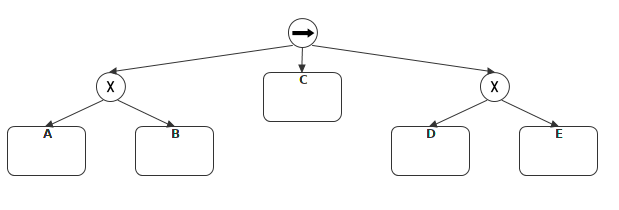
\includegraphics[width=\linewidth]{figures/algorithm/PT06_Seq_2_xor_notnested.png}
		\caption{The reviewed process tree PT}
		\label{fig:pt-lt-demo}
	\end{subfigure}%
	\quad
	\begin{subfigure}[b]{0.48\textwidth}
		\centering
		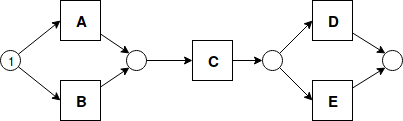
\includegraphics[width=\linewidth]{figures/algorithm/LT_Seq_01_Original.png}
		\caption{The reviewed Petri net}
		\label{fig:pn-lt-demo}
	\end{subfigure}%
\end{figure} 
% here we need to define the long-term dependency
%Based on the concepts above, we give a formal definition for long-term dependency in this thesis. 
%\begin{definition}[Long-term dependency for xor blocks] We call two xor blocks $S=\{X_1,X2,...X_m\}$ and $T=\{Y_1,Y_2,...Yn\}$ with long-term dependency, if 
%	 \[ S \prec T, d  \]
%\end{definition}
\subsubsection{Cases Analysis}
% Here we need to check the combination for all xor branches, but with one example.
There are various types  of long-term dependencies that are able to happen for two xor blocks. To explain those situations better, we define concepts called sources and targets of long-term dependency and then give an example of one Petri net with long-term dependency.
\begin{definition}[Source and target set of long-term dependency]
	The source set of the long-term dependency in two xor blocks is the set of all  xor branches, $LT_S:= \{X \vert \exists Y, X\rightsquigarrow Y  \in LT \} $, and target set is $LT_T:= \{Y \vert \exists X, X\rightsquigarrow Y \in LT \} $. \\
	For one xor branch $X \in S$, the target xor branch set relative to it with long-term dependency is 
	$ LT_T(X)= \{Y \vert  X\rightsquigarrow Y \in LT \}$
	Similarly, the source set related to one target xor branch is
	$ LT_S(Y)= \{X \vert  X\rightsquigarrow Y \in LT \}$
\end{definition}
At the same time, we use $S $ and $T$ to represent the set of xor branches for source and target xor block with long-term dependency.
Given a process tree in Figure \ref{fig:pt-lt-demo}, two xor blocks are contained in the model. They are able to have the following long-term dependencies.
% make it two graphs here, one is the process tree, one is the Petri net.
\begin{enumerate}
	\item $LT=\{ A\rightsquigarrow D, A\rightsquigarrow E, B\rightsquigarrow D, B\rightsquigarrow E\}$. \\
	$LT_S = \{A,B\}, LT_T=\{D,E\}, \vert LT \vert = \vert S \vert \cdot \vert T \vert  $, which is a full long-term dependency where all combinations of source and target xor branches have significant correlation. 
	\item $LT=\{ A\rightsquigarrow D, A\rightsquigarrow E, B\rightsquigarrow E\}. $\\
	$LT_S = \{A,B\}, LT_T=\{D,E\}$
	$LT_S = S $ and $LT_T = T, \vert LT \vert < \vert S \vert \cdot \vert T \vert $. it does not cover all combinations. But for one xor branch $X \in S, LT_T(X)= T$, it has all the full long-term dependency with $T$. 
	\item $LT=\{ A\rightsquigarrow D, B\rightsquigarrow E\}. $\\
	$LT_S = \{A,B\}, LT_T=\{D,E\}$
	$LT_S = S $ and $LT_T = T, \vert LT \vert < \vert S \vert \cdot \vert T \vert $. For all xor branch $X \in S, LT_T(X) \subsetneq T$, none of xor branch X has long-term dependency with $T$.
	\item $LT=\{ A\rightsquigarrow D, B\rightsquigarrow D\}.$ \\
	$LT_S = S ,  LT_T \subsetneq T$. There exists at least one xor branch $Y \in T$ which has no long-term dependency on it.
	\item $LT=\{ A\rightsquigarrow D, A\rightsquigarrow E\}.$ \\
	$LT_S \subsetneq S ,  LT_T = T$.
	There exists at least one xor branch in source $X \in S$ which has no long-term dependency on it.
	\item $LT=\{ A\rightsquigarrow E\}. $\\
	$LT_S \subsetneq S ,  LT_T \subsetneq T$.
	There exists at least one xor branch in source $X \in S$  and one xor target xor branch which has no long-term dependency on it.
	\item $LT=\emptyset$ . There is no long-term dependency on this set. 
\end{enumerate}
% here already to dispose several situations here and then 
%However, when the long-term dependency is full connected where each combination of xor branches from source and target xor block has long-term dependency, namely xor branches can be chosen freely, we do not add any places and silent transitions on the model.
In the listed situations, situation 1 is a full long-term dependency, which allows all combinations like the original models, and no changes are necessary on the model. Situation 7 has no long-term dependency, where the correlation of them is either not so strong from the positive instances or rejected from negative instances. In this thesis, we do not take those two situations into consideration.  

%% should we write down here to prove the correctness of available situations, or we need to wait??
\subsubsection{Way to Express Long-term Dependency}
% but how to come from the process tree to Petri net??? 
After detecting long-term dependencies with xor branches in process tree, it is not possible to express those dependencies on the process tree by using the current process tree operators. Moreover, the final output of our task demands a Petri net. Therefore, we convert the generated process tree into a Petri net and express long-term dependency on the Petri net with corresponding structures.

According to \cite{bergenthum2007process}, adding places to transitions in Petri net can limit the model behavior. Any transition demands a token from its input places to fire. When there is no token at this place, the transitions are not enabled. By adding extra places to the Petri net, it can block negative behaviors which are not expected in the aspect of business performance. 

Long-term dependency limits the available choices to fire transitions after the previous xor branch executes. So to express long-term dependency, our basic idea is to add places connected to transitions in the Petri net. In addition, because one xor branch can be as a source to multiple long-term dependencies and one xor branch can be as a target to multiple long-term dependencies, silent transitions are also needed to explicitly address a long-term dependency. 


Firstly, the long-term dependency set from process tree is mapped to the corresponding Petri net. For an arbitrary long-term dependency set $LT=\{X_i \rightsquigarrow Y_j \vert 1 \leq i \leq m, 1 \leq j \leq n \}$ with $S=\{X_1,X_2,...,X_m\}$ and $T=\{Y_1,Y_2,...,Y_n\}$ in a Petri net, we add places after the source xor branches in Petri net,  $P_S=\{p_{X_i} \vert X_i \in LT_{S} \}$, and places before target xor branches,$P_T=\{p_{Y_j} \vert Y_i \in LT_{T} \}$. For each long-term dependency $X_{i} \rightsquigarrow Y_{j}$ in LT, there is silent transition t with $p_{X_i} \rightarrow t \rightarrow p_{Y_{j}}$. The steps to add silent transitions and places according to the long-term dependency are listed in algorithm \ref{alg: Adding method}.

% An algorithm is given to show how to add the long-term dependency
\begin{algorithm}[!ht]
	\SetAlgoLined
	$Y$ is dependent on $X$\;
	\If{$X$ is leaf}{
		One place is added after this leaf\;
	}
	\If{$X$ is Seq}{
		Add a place after  the end node of this branch\;
		The node points to the new place\;
	}
	\If{$X$ is And}{
		Create a place after the end node of every children branch in this And xor branch\; 
		Combine all the places by a silent transition after those places\;
		Create a new place directly after silent transition to represent the And xor branch\;
	}
	
	\If{$Y$ is leaf}{
		One place is added before this leaf\;
	}\If{$Y$ is Seq}{
		Add a place before  the end node of this branch\;
		The new place points to this end node\;
	}\If{$Y$ is And}{
		Create a place before the end node of every children branch in this And xor branch\; 
		Combine all the places by a silent transition before those places\;
		Create a new place directly before silent transition to represent the And xor branch\;
	}
	Connect the places which represent the $X$ and $Y$ by creating a silent transition.
	\caption{Add long-term dependency between pure xor branch}
	\label{alg: Adding method}
\end{algorithm}
\begin{figure}
	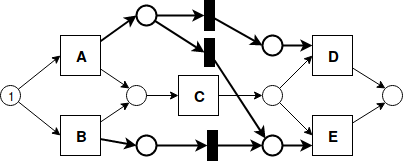
\includegraphics[width=\textwidth]{figures/algorithm/LT_Seq_01_Silent_01.png}
	\caption[Model with long-term dependency]{Model with long-term dependency $LT=\{ A\rightsquigarrow D, A\rightsquigarrow E, B\rightsquigarrow E\}. $ }
	\label{fig:pn-demo-with-lt}
\end{figure}
Reviewing the example of process tree of Figure \ref{fig:pt-lt-demo}, it has long-term dependency set $LT=\{ A\rightsquigarrow D, A\rightsquigarrow E, B\rightsquigarrow E\}$. To express long-term dependency,  the process tree is firstly transformed into the Petri net as Figure \ref{fig:pn-lt-demo}. Then two extra places are added respectively after A and B; Next, two places before D and E are created to express that the xor branches are involved with long-term dependency. At end, for each long-term dependency, a silent transition is generated to connect the extra places after the source xor branch to the place before target place. The generated model with long-term dependency is displayed in Figure \ref{fig:pn-demo-with-lt}.

\subsubsection{Soundness Analysis}
% this section is used to select the sound situations. 
% next time I can go to library at Tuesday with the laptop and study there..
With Algorithm \ref{alg: Adding method} by adding silent transitions and places to express long-term dependency, the model soundness can be violated. In the following section, we discuss the soundness in different situations. 

Given a Petri net with long-term dependency $LT=\{X_i \rightsquigarrow Y_j \vert 1 \leq i \leq m, 1 \leq j \leq n \}$ on two xor blocks $S=\{X_1,X_2,...X_m\}$ and $T=\{Y_1,Y_2,...Y_n\}$. After applying the Algorithm \ref{alg: Adding method}, $P_S=\{p_{X_i} \vert X_i \in LT_{S} \}$ , $P_T=\{p_{Y_j} \vert Y_i \in LT_{T} \}$, and silent transitions $ E = \{\epsilon \vert p_{X_i} \rightarrow \epsilon
\rightarrow p_{Y_{j}} \}$ are added. 
 
The Petri net is sound if and only if (1) the soundness outside xor blocks with long-term dependency is not violated; and  (2) soundness between xor blocks is kept. In the following, we check the model soundness with long-term dependency after applying Algorithm \ref{alg: Adding method}. \\\\
\textbf{Soundness outside xor blocks.}\\
	\emph{Proof:} The added silent transitions and places do not violate the execution outside of the xor blocks, because the extra tokens that are generated due to long-term dependency are constrained in the xor blocks, and it does not affect the token flows outside. As we know, the original model is sound. So the soundness outside xor blocks is not violated.
%% begin to prove the soundness inside xor block
\\\\
\textbf{Soundness inside xor blocks.}\\
For the xor blocks $S=\{X_1,X_2,...X_m\}$ and $T=\{Y_1,Y_2,...Y_n\}$ with long-term dependency $LT=\{X_i \rightsquigarrow Y_j \vert 1 \leq i \leq m, 1 \leq j \leq n \}$, only one xor branch can be fired in S. Without loss of generality, $X_i$ is assumed to be enabled. After firing $X_i$, the marking distribution on the extra places are  
\[ M(p_{X_i}) = 1; \quad 
\forall p_{X_{i^\prime}} \in P_S, i^\prime \neq i, M(p_{X_{i^\prime}})=0 \]
%% here we need to divide them into different situations...
If $ LT_S = S, LT_T=T$, adding the long-term dependency in this situation does not violate the model soundness, we prove it in the following part.
%the following conditions are checked. 
\begin{itemize}
	\item Safeness. Places cannot hold multiple tokens at the same time.\\
	For all extra places $p_{X_i}$ and $p_{Y_j}$, 
	\[\forall p_{X_i} \in P_S, \sum M(p_{X_i})=1\]
	Because $ LT_S = S, X_i \in S$, so $X_i \in LT_S$, there exists one $Y_j$ with $X_i \rightarrow Y_j$ and one $\epsilon, p_{X_i} \rightarrow \epsilon
	\rightarrow p_{Y_{j}} $.  After firing $X_i$, the transition $\epsilon$ becomes enabled. After executing $\epsilon$, the marking distribution turns to 
	\[ M(p_{Y_j}) = 1;\quad 
	\forall p_{Y_j^\prime} \in P_T, j^\prime \neq j,  M(p_{Y_i})=0 \]
	the marking distribution in the extra places are always
	\[\sum M(p_{X_i}) \leq 1,  \sum M(p_{Y_j}) \leq 1 \] 
	\item Proper completion. If the sink place is marked, all other places are empty. \\
	After firing $Y_j$, all the extra places hold no token. So it does not violate proper completion.
	\item Option to complete.  It is always possible to reach the final marking just for the sink place. \\
	There is always one $Y_j$ enabled after firing $X_i$ to continue the subsequent execution.
	\item No dead part. For any transition there is a path from source to sink place. \\
	Because all $Y_j \in T$ are also in $LT_T$, there exists at least one $X_i\in S$ with long-term dependency with $Y_j$. After $X_i$ is fired, one token is generated on the extra place $p_{X_i}$ and can be consumed by silent transition $\epsilon$ in  $p_{X_i} \rightarrow \epsilon \rightarrow p_{Y_{j}}$ to produce a token in $p_{Y_j}$, which enables xor branch $Y_j$ and leaves no dead part.
\end{itemize}
In other situation, the model becomes unsound. \\
\indent If $LT_S \neq S$, or $\quad LT_T \neq \emptyset$, there exists one xor branch $X_i$ with $X_i \notin LT_S$. When $X_i$ is fired, it generates one token at place $p_{X_i}$, this token cannot be consumed by any $Y_j$. So it violates the proper completion. \\  
\indent If $LT_T \neq T$, there exists one $Y_j \notin LT_T, \nexists X_i, X_i \rightsquigarrow Y_j$, so with two input places but $Token(p_{Y_j})=0$,  $Y_j$ becomes a dead part, which violates soundness again. 
As a conclusion, to keep Petri net with long-term dependency sound, only situations with $ LT_S = S, LT_T=T$ are considered.  
\subsection{Reduce Silent Transitions}
%% We reduce the silent transition when there is no 
Our method to represent long-term dependency can introduce redundant silent transitions and places, which complicates the model. So, we post process the Petri net with long-term dependency and delete redundant silent transitions and places in it. 
% definition of redundant transitions and places
Silent transitions and places of a Petri net are redundant when the Petri net preserves the behavior without those transitions and places \cite{murata1989petri, verbeek2017decomposed}. There is an existing algorithm developed in the work of \cite{verbeek2017decomposed}. We reuse it as one post process in our thesis. 

%% here we need to prove this proposition
One example is given in the following graph. $M_{lt}$ in Figure \ref{fig:with-lt} has long-term dependency expressed in the silent transitions and places. The silent transition for $S2 \rightsquigarrow B1 $ and silent transition for $B1 \rightsquigarrow T2$ belongs to the case (1). So they are kept in the model, while the other silent transitions are deleted. After reducing the redundant silent transitions, the model becomes $M_r$ shown in Figure \ref{fig:reduced-lt}. Those two models have the same behavior, yet the reduced model is simpler.
\begin{figure}[!h]
	\centering
	\begin{subfigure}[a]{\textwidth}
		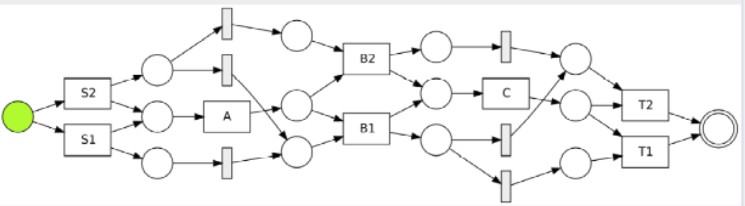
\includegraphics[width=\textwidth]{figures/algorithm/dfg-IM-pn-with-lt.png}
		
		\caption{A Petri net $M_{lt}$ with redundant silent transitions}
		\label{fig:with-lt}
	\end{subfigure}
	\hfill
	\begin{subfigure}[b]{\textwidth}
		\centering
		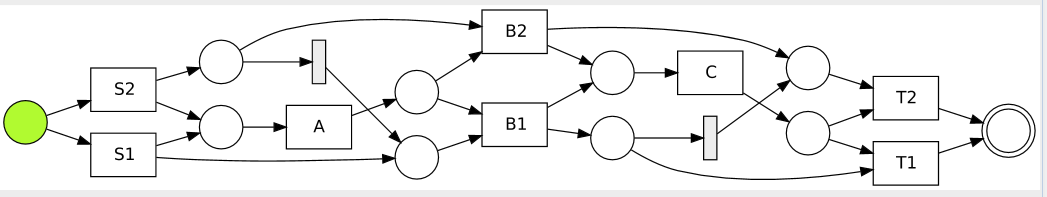
\includegraphics[width=\linewidth]{figures/algorithm/dfg-IM-pn-with-lt-reduced.png}
		
		\caption{Petri net $M_r$ with reduced silent transitions}
		\label{fig:reduced-lt}
	\end{subfigure}
\end{figure}
\subsection{Concrete Architecture}
At last, we assemble all the modules together and give an overview architecture of our repair techniques.  We reuse existing modules in gray rectangles in Figure \ref{fig:architecture}, e.g. IMLog2Dfg to convert an event log into directly-follow graph, Petrinet2TransitionSystem to transform a Petri net into a transition system. The other modules are programmed according to our specific needs and achieve the repair algorithm mentioned before. To achieve a more precise Petri net, the module to add long-term dependency becomes a necessary part. Yet, reduction on redundant places and silent transitions is optional. 
\begin{figure}
	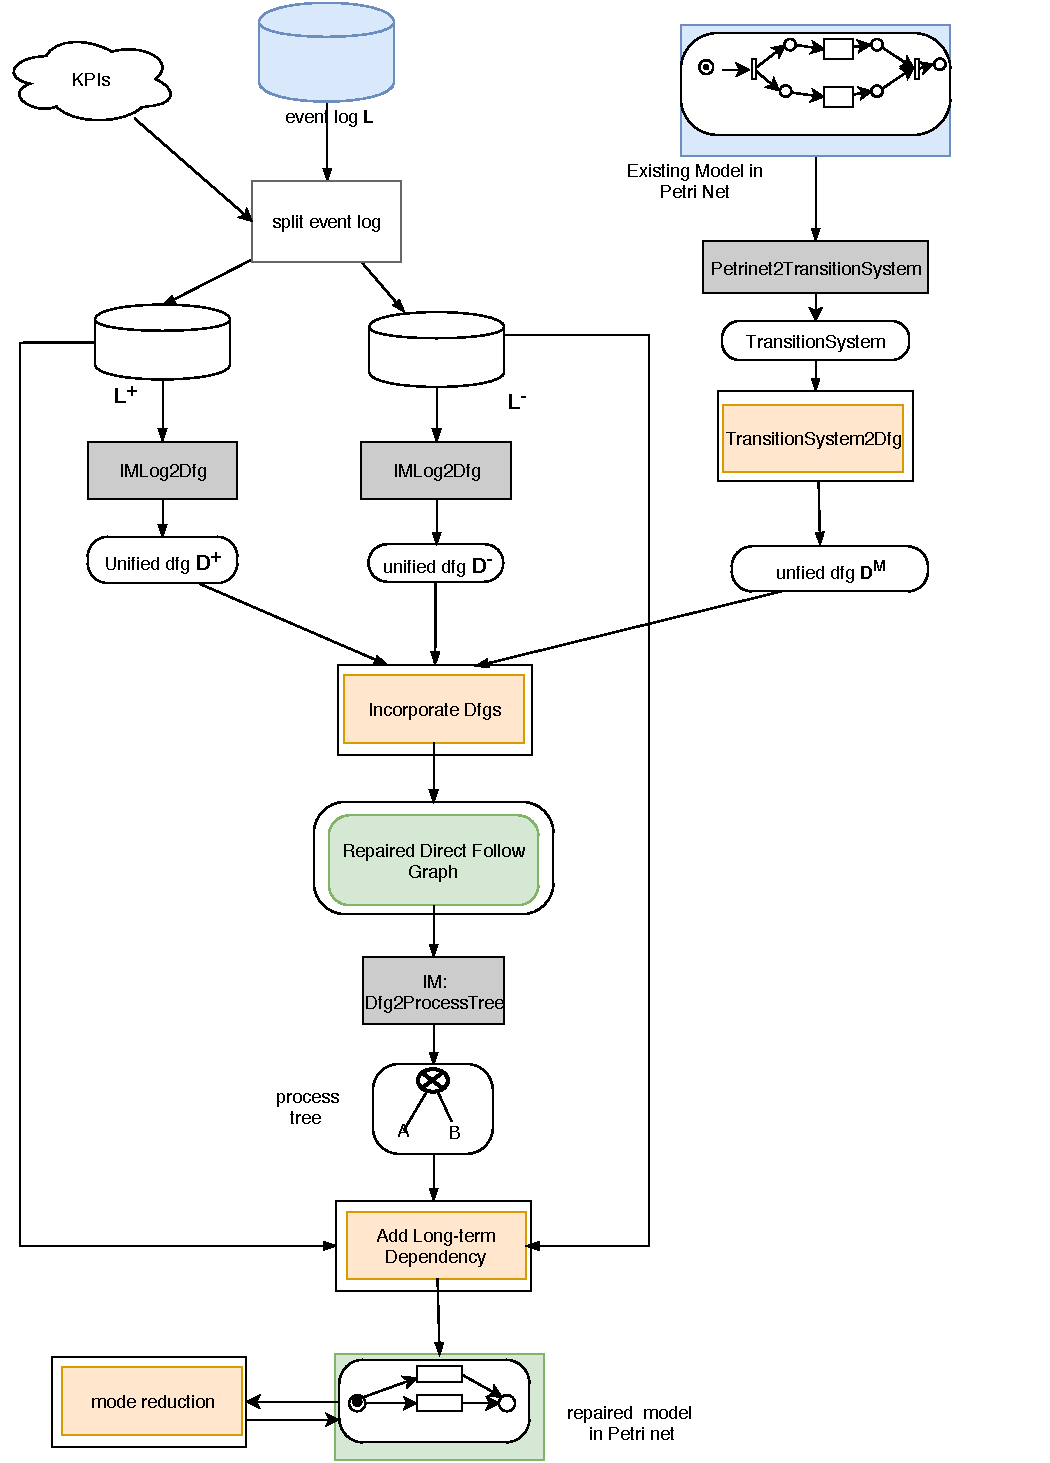
\includegraphics[height=0.9\textheight]{figures/algorithm/FD_architeccture_details.pdf}
	\caption[Model Repair Architecture]{Model Repair Architecture -- \small Rectangles represents processes and output data in eclipse shape, especially customized processes and data are in doubled eclipses. Input event log and existing model are in blue, KPIs are in cloud. The output is a petri net in green.}
	\label{fig:architecture}
\end{figure} 
